\documentclass[conference]{IEEEtran}
\usepackage{cite}
\usepackage{amsmath,amssymb,amsfonts}
\usepackage{algorithmic}
\usepackage{graphicx}
\usepackage{textcomp}
\usepackage{xcolor}
\usepackage{booktabs}
\usepackage{tabularx}
\usepackage{url}
\usepackage{float}
\usepackage{subcaption}

\begin{document}

\title{Do Voters Reward Fiscal Performance?\\ 
\Large A Machine Learning and Causal Analysis of Philippine Gubernatorial Elections}

\author{\IEEEauthorblockN{Jemar John J. Lumingkit}
\IEEEauthorblockA{\textit{Mindanao State University---Iligan Institute of Technology} \\
Email: jemar.lumingkit@g.msuiit.edu.ph}
}

\maketitle

\begin{abstract}
Do voters reward governors for better health and education spending, increased local revenue, and lower IRA dependence? Using a panel of Philippine provinces (1992–2022) and an XGBoost classifier, we predict gubernatorial re‑election based on fiscal performance, political competition, dynasty status, and previous vote margin. With 5‑fold stratified cross‑validation, the model achieves a mean accuracy of 92.0\% (SD 0.8\%) and an ROC‑AUC of 0.977 (SD 0.006). SHAP analysis shows that education and health spending growth are top predictors. A dynasty‑by‑health interaction term appears in the top ten features (gain importance 0.044, mean SHAP 0.020), indicating that dynastic incumbents receive a small positive electoral reward for health spending increases. Temporal validation (training on pre‑2016 data and testing on 2019–2022) shows poor generalisation (accuracy 44.3\%), suggesting electoral dynamics change over time. Regression discontinuity estimates a positive but fragile effect of winning on health spending (ATE = 1.50, 95\% CI [0.07, 2.94]). All provinces in the dataset belong to income class 3, preventing a rich‑poor subgroup analysis. The results align with SDG 16 (accountable governance) and SDG 4 (quality education).
\end{abstract}

\begin{IEEEkeywords}
Fiscal performance, gubernatorial elections, XGBoost, regression discontinuity, accountable governance, Philippines.
\end{IEEEkeywords}

\section{Introduction}

The 1991 Local Government Code devolved substantial responsibilities to Philippine local governments, giving governors significant control over health, education, and infrastructure budgets. In theory, voters can hold incumbents accountable by rewarding those who deliver better services and penalizing those who do not. Yet empirical evidence on whether fiscal performance actually influences re‑election is limited, especially using modern machine learning methods.

This study uses an XGBoost classifier to predict whether an incumbent governor wins re‑election based on:
\begin{itemize}
\item Growth in health and education spending per capita
\item Local revenue per capita
\item Political competition (effective number of candidates, ENC)
\item Dynasty status (whether the incumbent shares a surname with the previous governor)
\item Previous election margin
\item Income class and region
\end{itemize}

We also implement a regression discontinuity design (RDD) on close elections to estimate the causal effect of winning on subsequent health spending growth, and we include interaction terms to test whether fiscal accountability differs between dynastic and non‑dynastic incumbents.

\section{Data and Variables}

\subsection{Data Sources}
We combine two primary datasets:
\begin{itemize}
\item \textbf{Fiscal panel} (1992–2022): 227 LGUs, annual spending on health, education, local revenue, IRA share, ENC, dynasty indicator (constructed from incumbent surnames).
\item \textbf{Election results} (1992–2022): gubernatorial vote shares, winners, and turnout.
\end{itemize}
Population data from the Philippine Statistics Authority (censuses 1995–2024) are interpolated to yearly estimates to compute per‑capita spending.

The fiscal and election data are taken from the Philippine Local Government Interactive Dataset \cite{b5}.

\subsection{Data Cleaning and Preparation}
The raw fiscal data contain annual LGU records (1992–2022) with spending on health, education, public welfare, etc. For each LGU and election year, we identify the start of a term (fiscal year equals election year) and retain the incumbent governor’s name, fiscal variables (IRA share, local revenue, ENC), and pre‑term spending averages (three years before the election). Using the election file, we compute vote shares, winners, and the candidate’s name. We then merge the two datasets on LGU and election year to obtain, for each term, the incumbent’s electoral outcome.

To construct the dynasty indicator, we compare the incumbent’s surname with the previous term’s incumbent (same LGU) and assign 1 if they match. Population data from five censuses (1995–2024) are interpolated linearly to obtain yearly estimates for 1992–2022. Per‑capita spending is computed by dividing nominal spending (converted from millions to pesos) by the interpolated population. Growth rates for health, education, and local revenue are calculated as \((\text{post} - \text{pre}) / \text{pre}\), clipped to \([-0.9, 5]\) to avoid extreme outliers. Finally, we keep only terms where the incumbent ran for re‑election (i.e., the winner of term \(t\) also contested term \(t+3\)) and create the target variable `won` (1 if the same person won the next election, 0 otherwise). Missing previous vote margins are filled with 0.5 (neutral). The final dataset contains 1,682 observations (787 re‑elected, 895 defeated).

\subsection{Variables}
For each incumbent who ran for re‑election, we compute:

\begin{table}[H]
\caption{Features and target}
\centering
\begin{tabular}{ll}
\toprule
Feature & Description \\
\midrule
$\Delta$health & (health spending per capita in post‑term years) / (pre‑term) – 1 \\
$\Delta$educ   & same for education \\
$\Delta$local\_rev & same for local revenue per capita \\
enc\_gol & effective number of candidates (political competition) \\
dynasty & 1 if incumbent shares surname with previous governor, else 0 \\
prev\_margin & incumbent’s vote share in the previous election \\
income\_class & 1 (richest) to 6 (poorest) – all observations are class 3 \\
region & 17 regions (one‑hot encoded) \\
\midrule
\textbf{Target} & \textbf{won} = 1 if re‑elected, 0 otherwise \\
\bottomrule
\end{tabular}
\end{table}

\section{Methodology}

\subsection{Predictive Model (XGBoost)}
We use an \textbf{XGBoost classifier} with 200 trees, maximum depth 5, learning rate 0.05, and subsample/colsample by tree 0.8. Model evaluation is performed using 5‑fold stratified cross‑validation. Feature importance is extracted using SHAP (SHapley Additive exPlanations) values \cite{b9}. To explore heterogeneity, we add interaction terms (dynasty $\times$ $\Delta$educ, dynasty $\times$ $\Delta$health).

\subsection{Temporal Validation}
We perform a temporal robustness check: train on elections up to 2016, test on 2019–2022.

\subsection{Regression Discontinuity Design (RDD)}
To address endogeneity, we exploit close elections. The running variable is the incumbent’s vote margin (vote share – 0.5). The treatment is winning (margin > 0). The outcome is health spending growth after the term. We use local linear regression with a triangular kernel and bandwidths of 3\%, 5\%, and 7\% of the margin. The 5\% bandwidth is the primary specification.

\section{Results}

\subsection{Model Performance (Cross‑Validation)}
Table I reports the 5‑fold cross‑validation results for XGBoost. The model achieves a mean accuracy of 92.0\% (SD 0.8\%) and a mean AUC of 0.977 (SD 0.006), with precision, recall, and F1 scores all above 0.91.

\begin{table}[H]
\caption{5‑fold cross‑validation results for XGBoost}
\centering
\begin{tabular}{lccccc}
\toprule
Fold & Accuracy & AUC & Precision & Recall & F1 \\
\midrule
1 & 0.935 & 0.985 & 0.915 & 0.949 & 0.932 \\
2 & 0.911 & 0.970 & 0.932 & 0.873 & 0.902 \\
3 & 0.917 & 0.982 & 0.877 & 0.955 & 0.915 \\
4 & 0.923 & 0.979 & 0.912 & 0.924 & 0.918 \\
5 & 0.914 & 0.971 & 0.927 & 0.885 & 0.906 \\
\midrule
\textbf{Mean} & \textbf{0.920} & \textbf{0.977} & \textbf{0.913} & \textbf{0.917} & \textbf{0.914} \\
\textbf{SD} & \textbf{0.008} & \textbf{0.006} & \textbf{0.020} & \textbf{0.035} & \textbf{0.012} \\
\bottomrule
\end{tabular}
\end{table}

For comparison, Table II presents the cross‑validated performance of baseline models. XGBoost substantially outperforms logistic regression (accuracy 62.7\%, AUC 0.663) and random forest (accuracy 73.9\%, AUC 0.853). LightGBM achieves close performance (accuracy 90.3\%, AUC 0.969) but remains slightly inferior to XGBoost.

\begin{table}[H]
\caption{Comparison of baseline models (5‑fold CV)}
\centering
\begin{tabular}{lcc}
\toprule
Model & Accuracy (mean) & AUC (mean) \\
\midrule
Logistic Regression & 0.627 & 0.663 \\
Random Forest & 0.739 & 0.853 \\
LightGBM & 0.903 & 0.969 \\
\bottomrule
\end{tabular}
\end{table}

The ROC curve (Fig. 1) from a representative fold confirms excellent separation.

\begin{figure}[H]
\centering
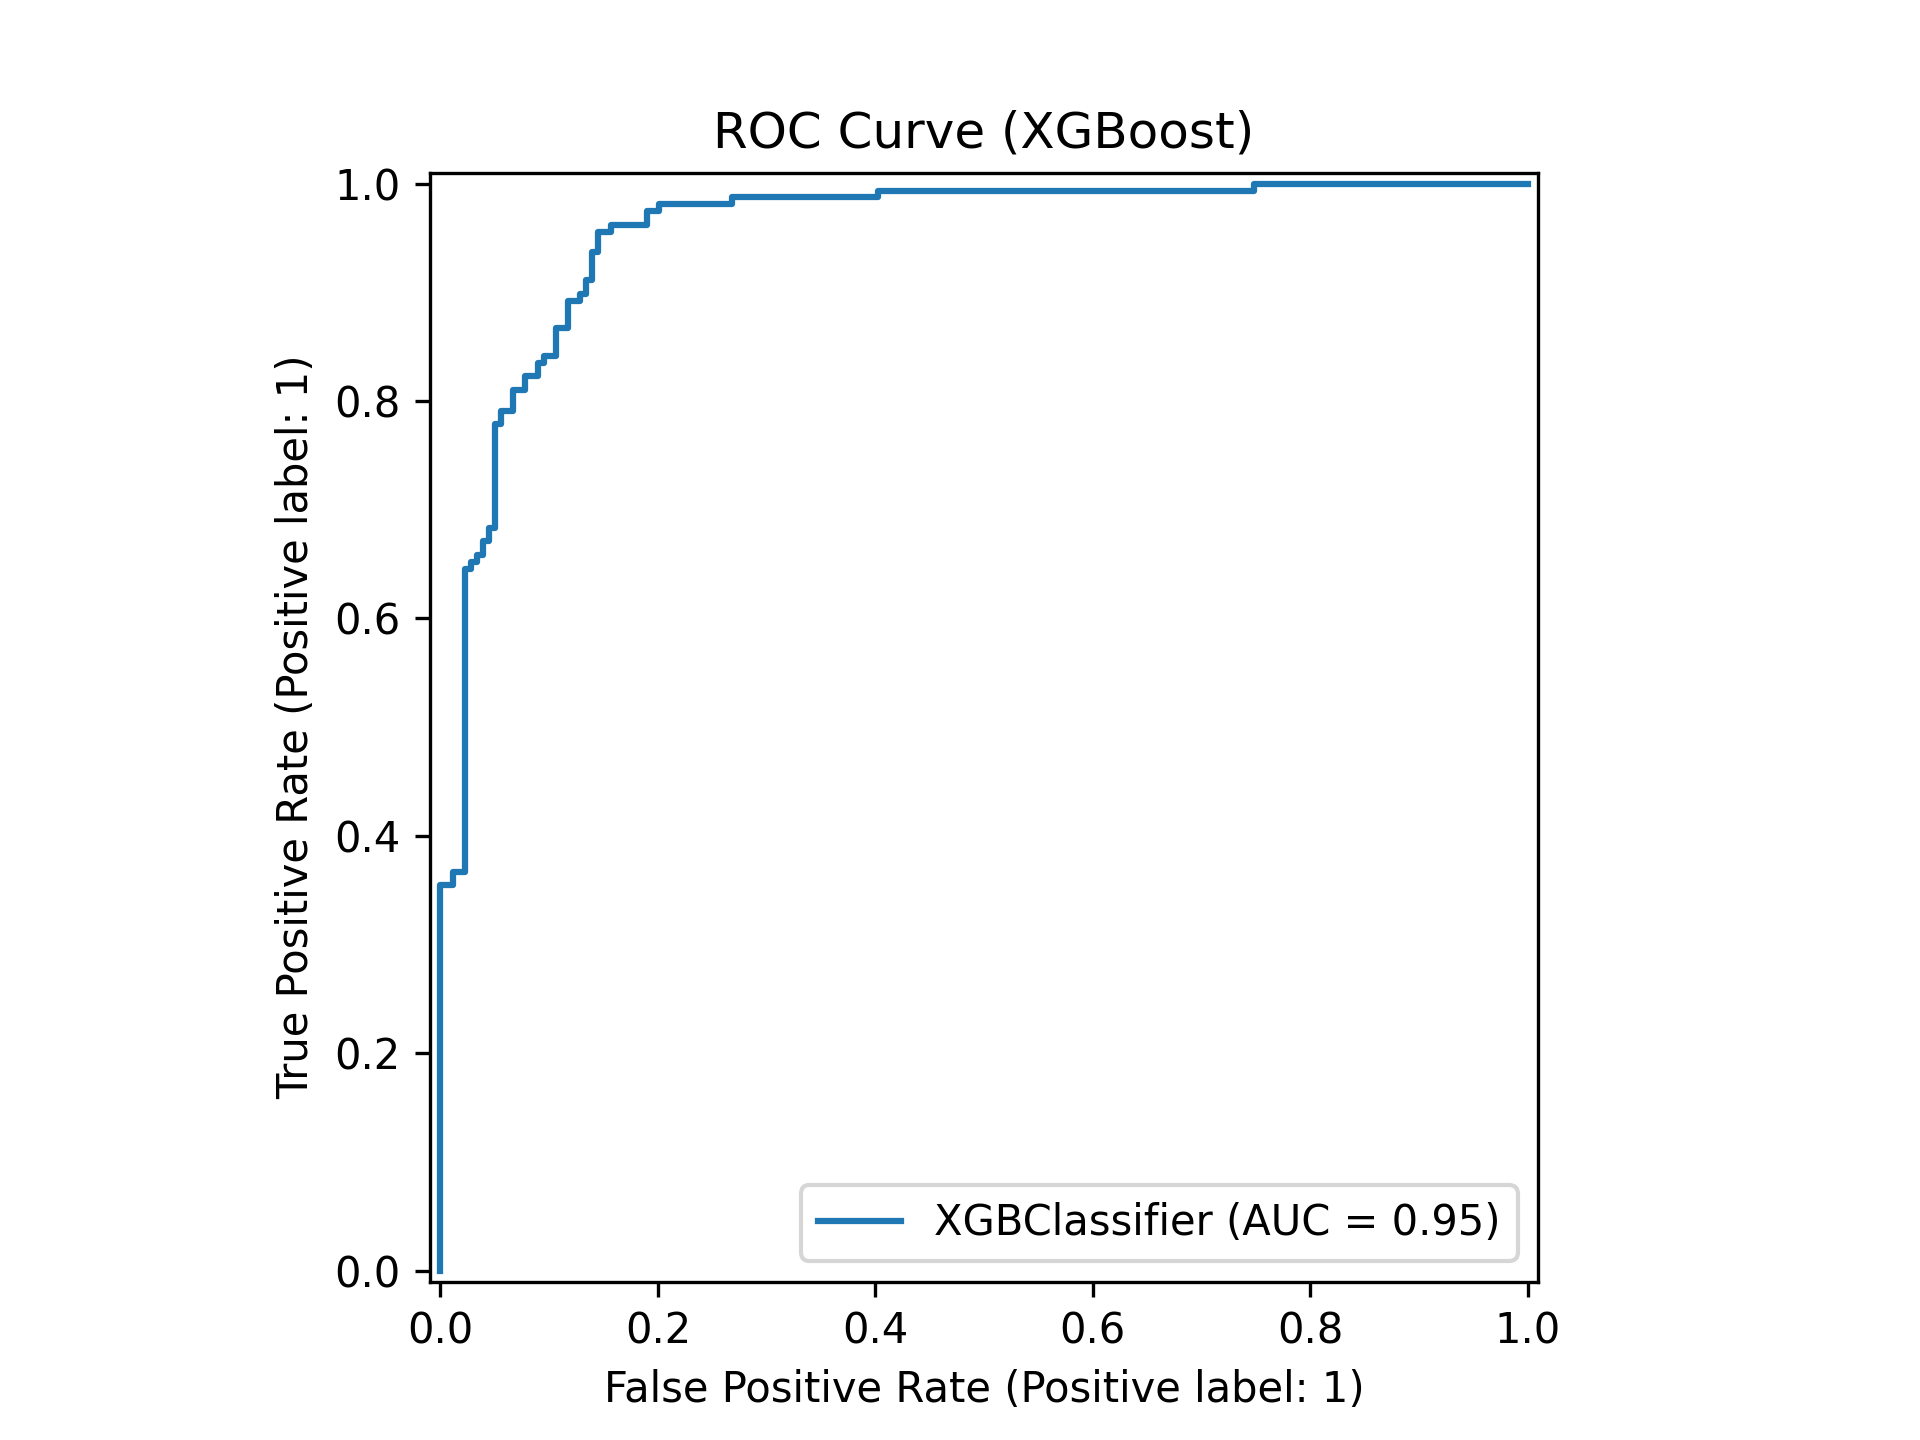
\includegraphics[width=0.9\columnwidth]{../data/roc_curve.png}
\caption{ROC curve (random split example).}
\label{fig:roc}
\end{figure}

\subsection{Correlation Analysis}
Figure 2 shows the correlation between numeric features and the target. Health spending growth, education spending growth, and local revenue per capita are positively correlated with re‑election.

\begin{figure}[H]
\centering
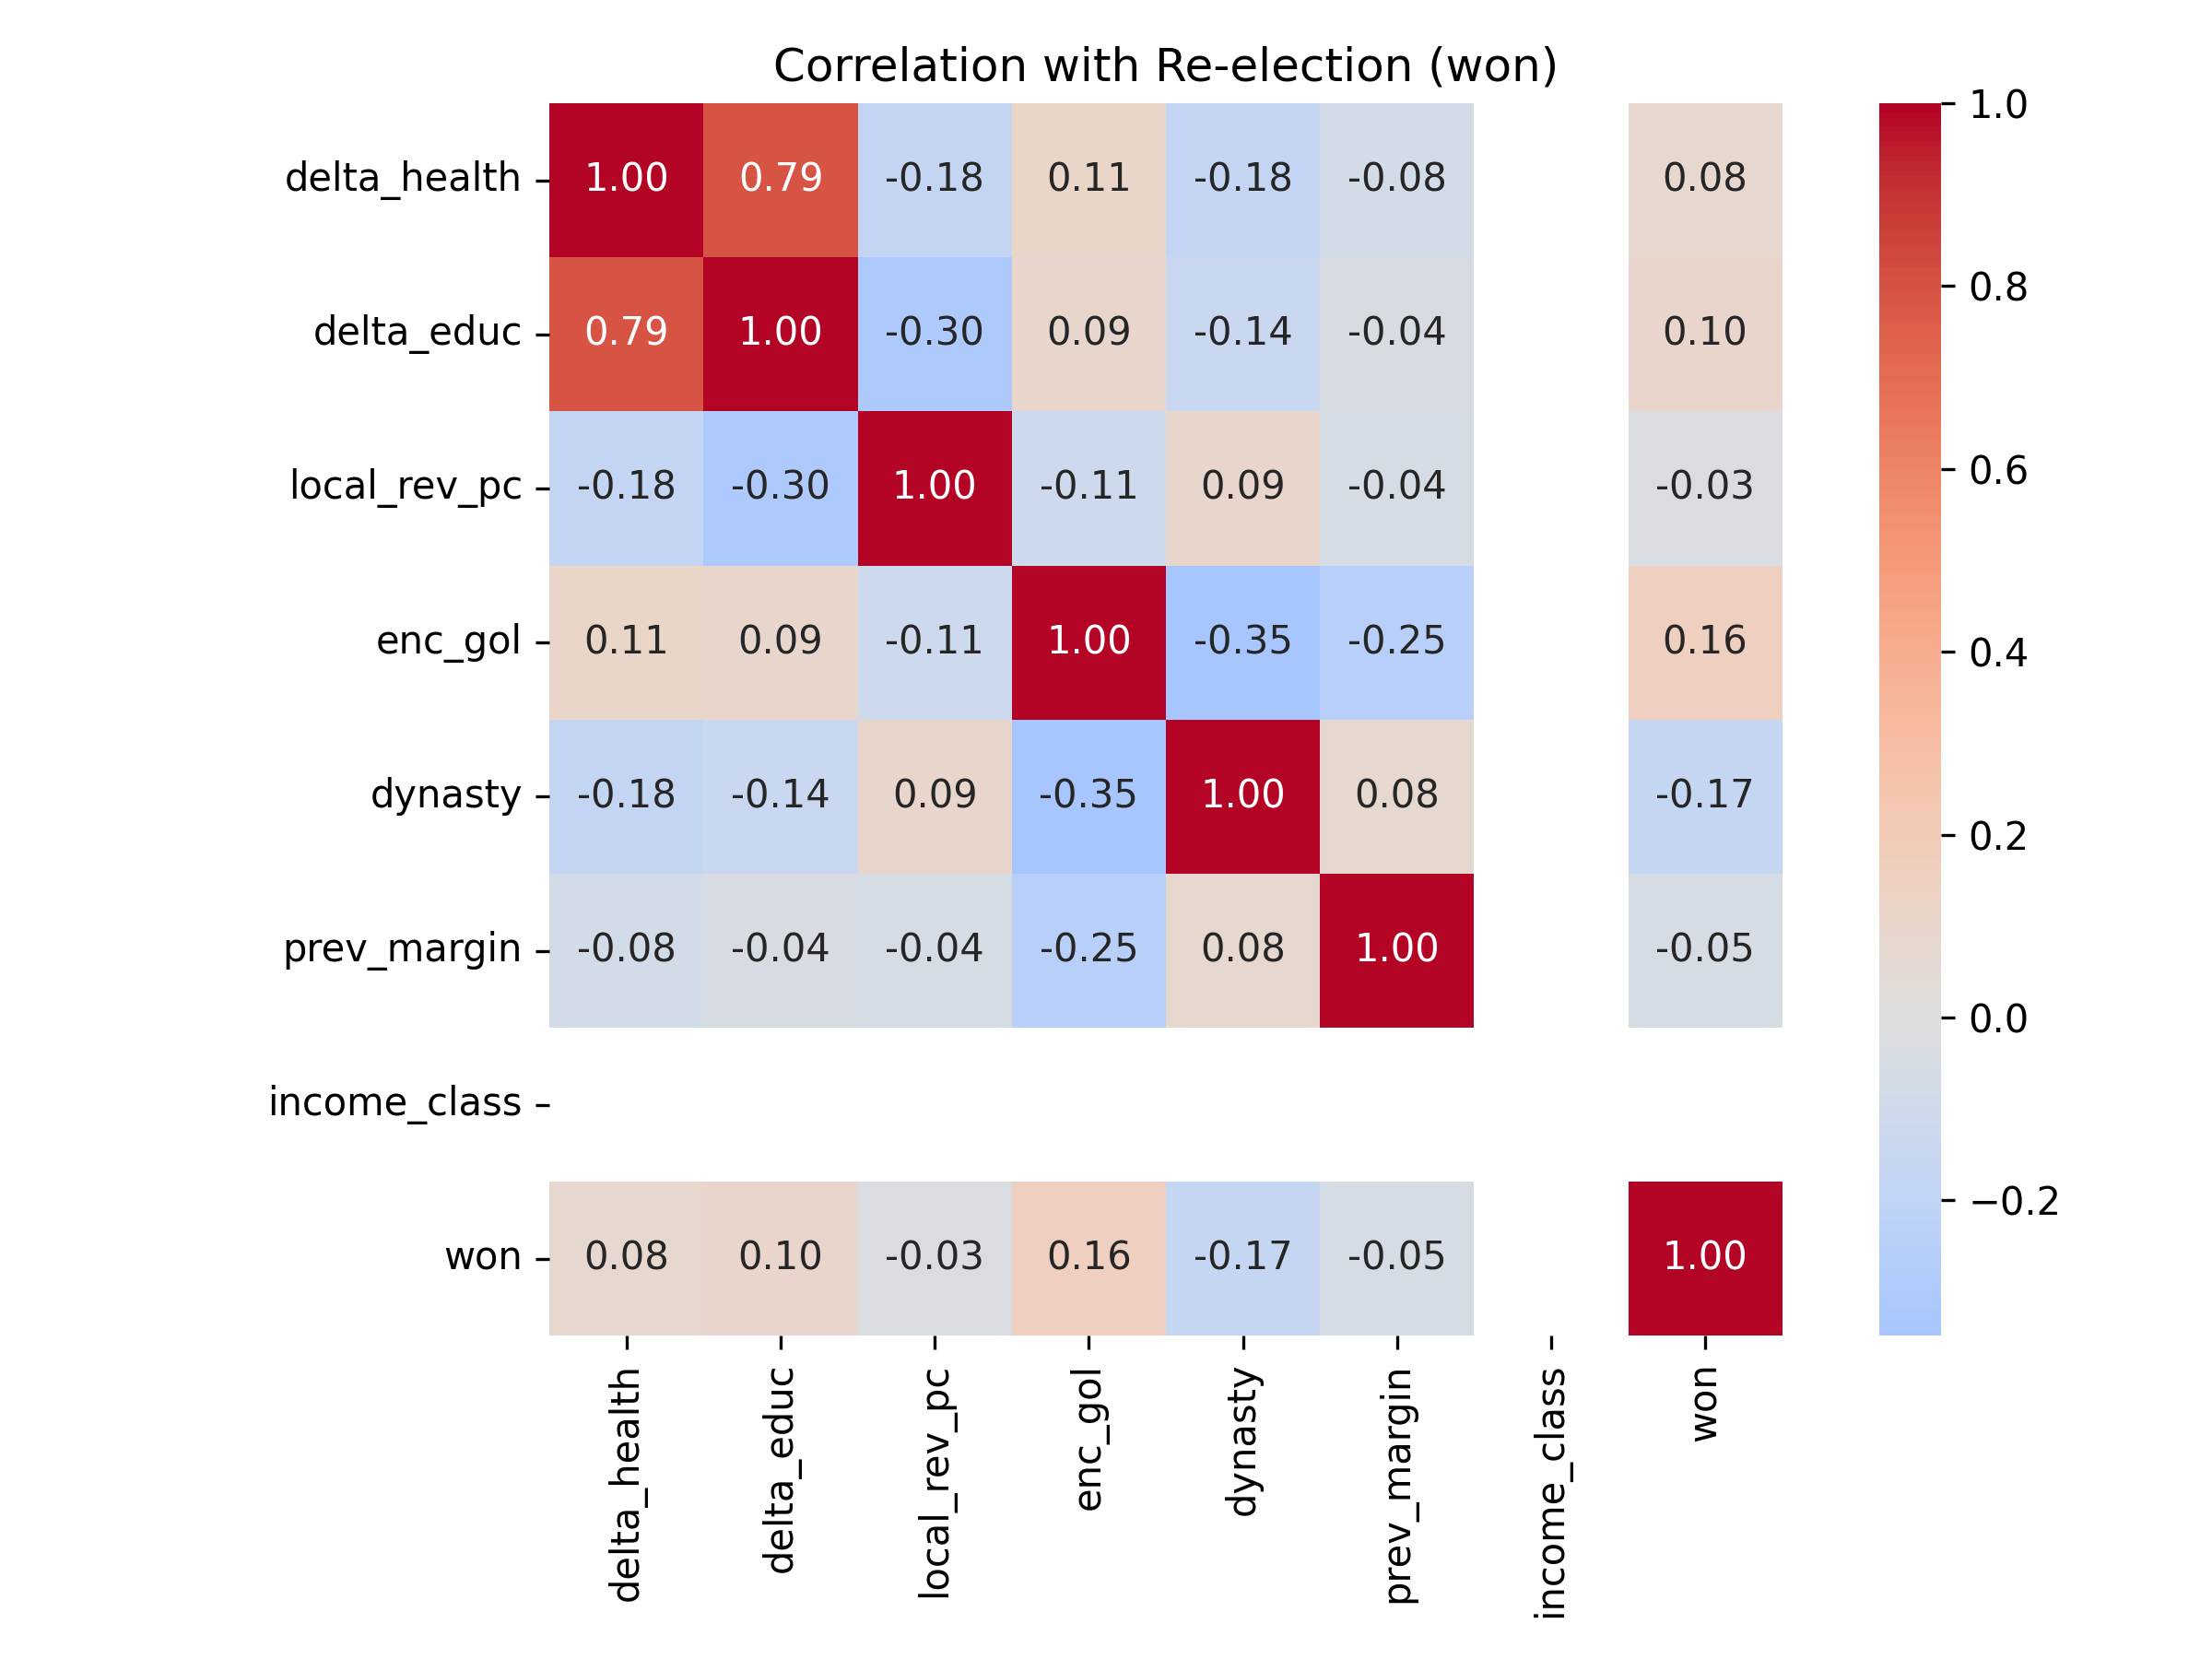
\includegraphics[width=0.9\columnwidth]{../data/correlation_heatmap.png}
\caption{Correlation heatmap of numeric features with re‑election.}
\label{fig:corr}
\end{figure}

\subsection{Feature Importance (SHAP)}
Figure 3 shows the SHAP bar plot (mean absolute SHAP values). Education spending growth ($\Delta$educ), political competition (enc\_gol), and health spending growth ($\Delta$health) are the most important numeric predictors after region fixed effects. The mean absolute SHAP for $\Delta$educ is 0.363, for enc\_gol 0.460, and for $\Delta$health 0.326.

\begin{figure}[H]
\centering
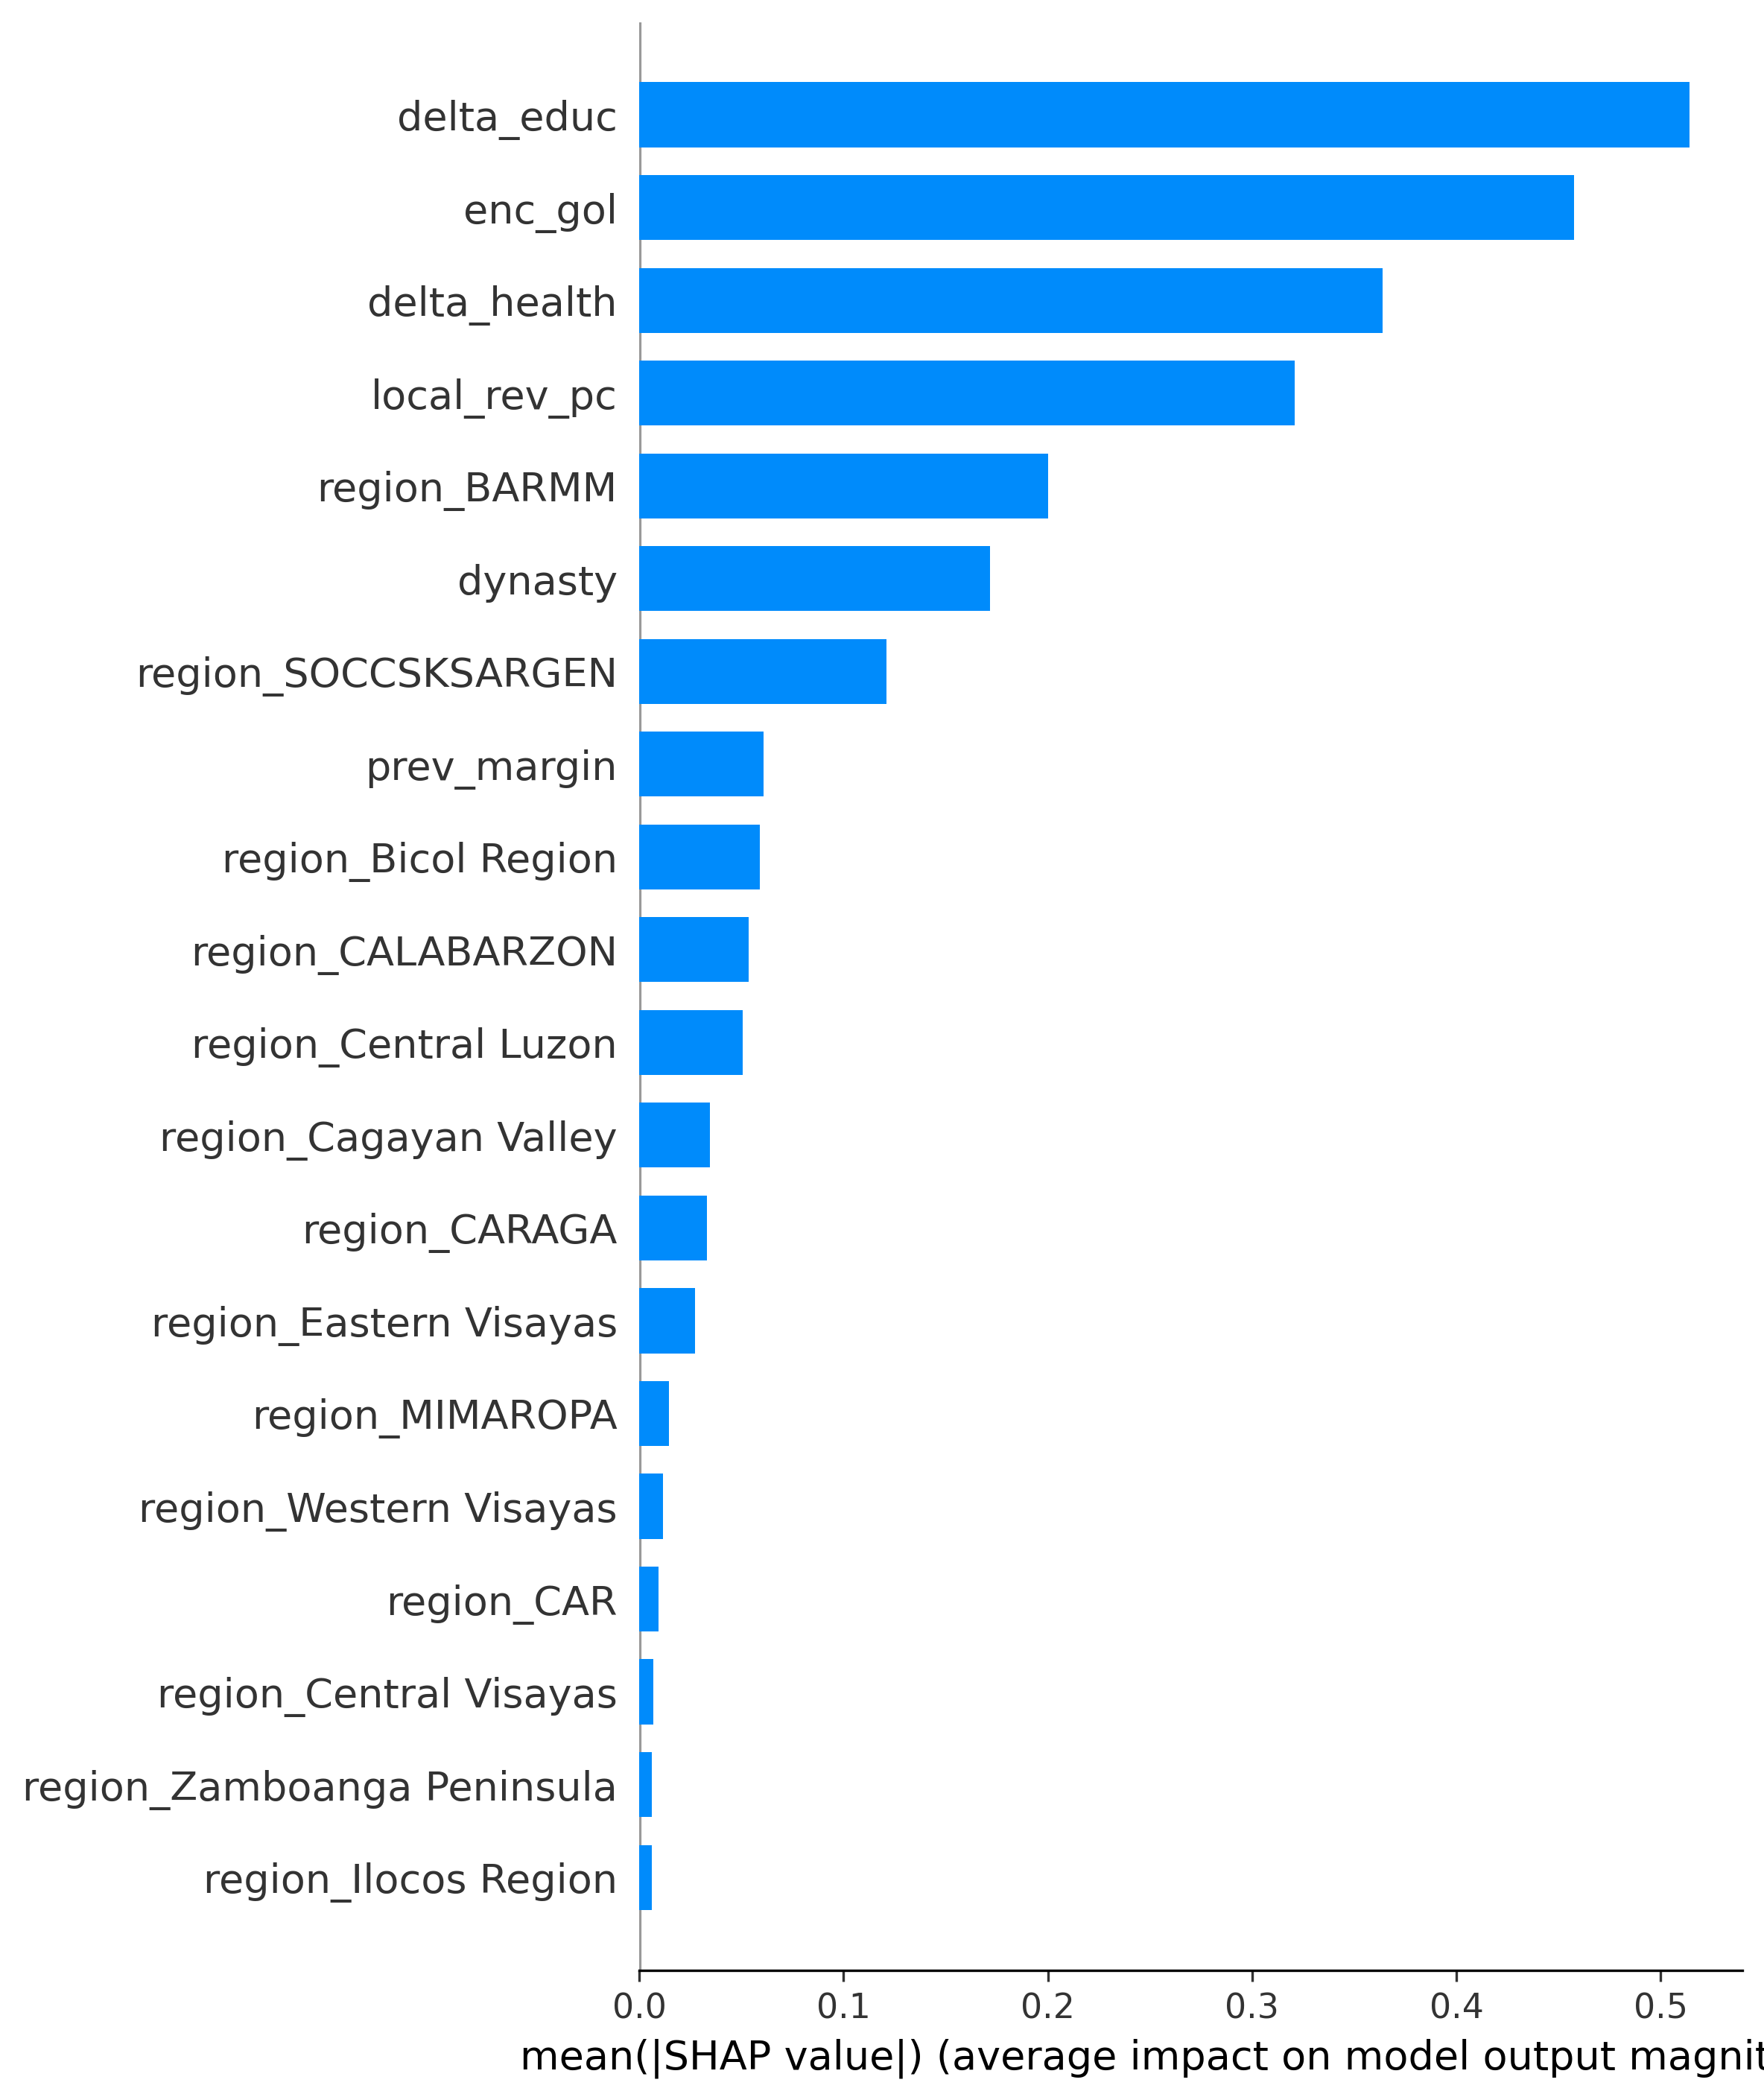
\includegraphics[width=0.9\columnwidth]{../data/shap_bar.png}
\caption{SHAP bar plot (mean absolute SHAP values).}
\label{fig:shap_bar}
\end{figure}

\subsection{SHAP Dependence Analysis}
Figures 4a and 4b show the SHAP dependence plots for education growth ($\Delta$educ) and health growth ($\Delta$health). The SHAP value increases with higher growth rates, indicating that voters reward governors who raise per‑capita education and health spending.

\begin{figure}[H]
\centering
\begin{subfigure}{0.48\columnwidth}
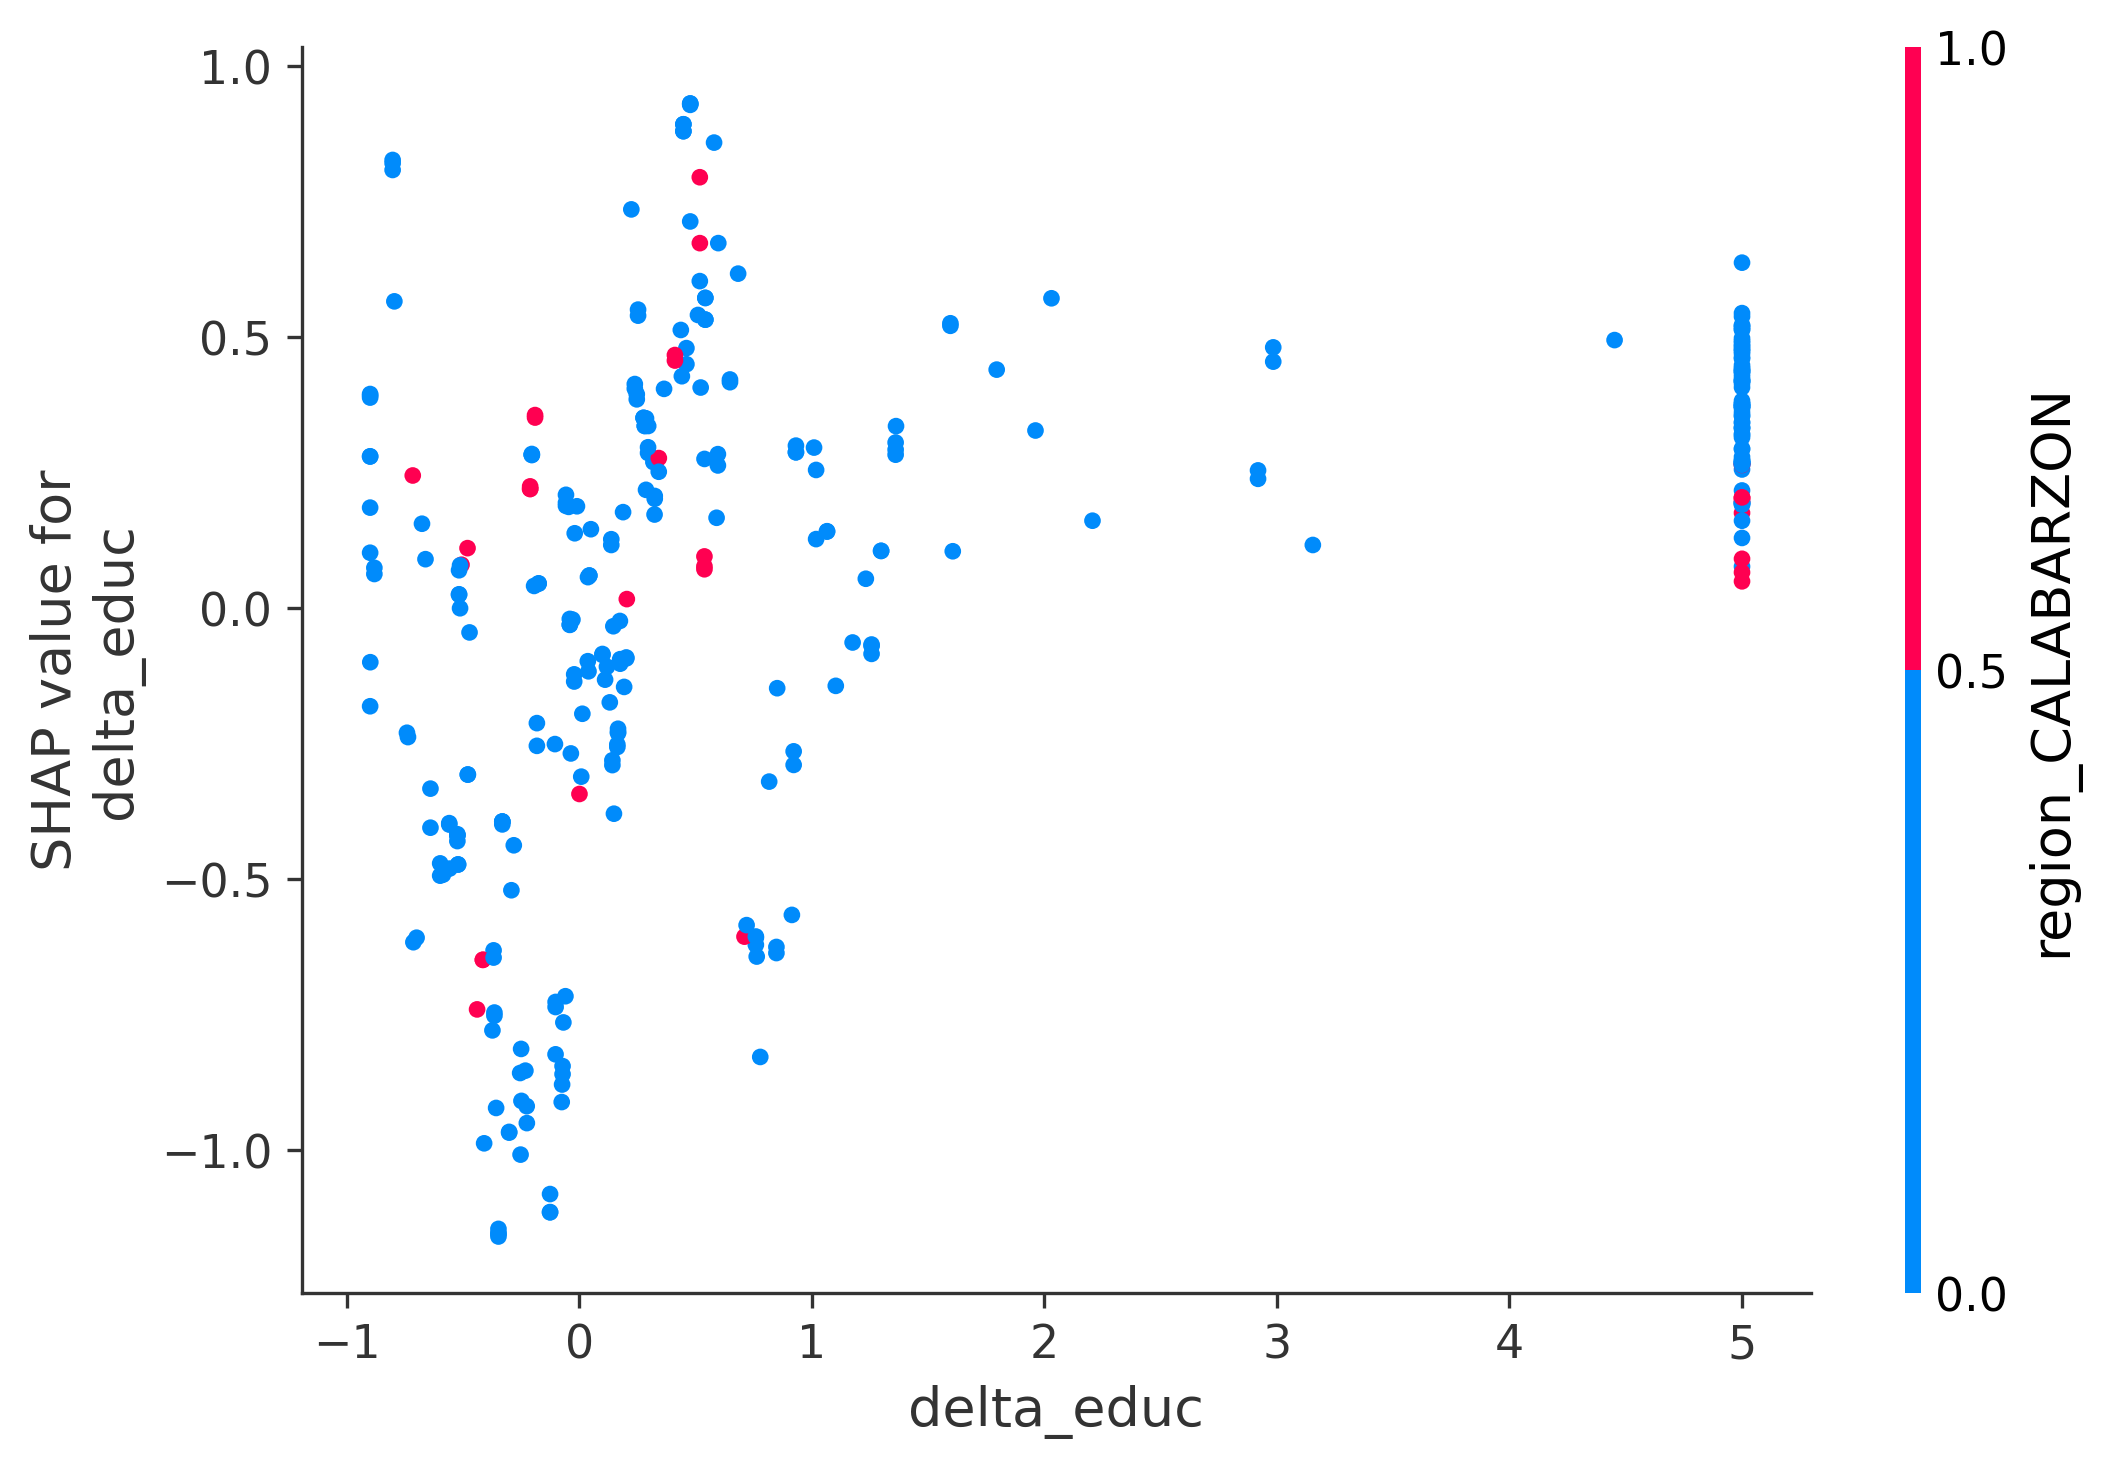
\includegraphics[width=\linewidth]{../data/shap_dependence_educ.png}
\caption{SHAP dependence for $\Delta$educ.}
\label{fig:shap_educ}
\end{subfigure}
\hfill
\begin{subfigure}{0.48\columnwidth}
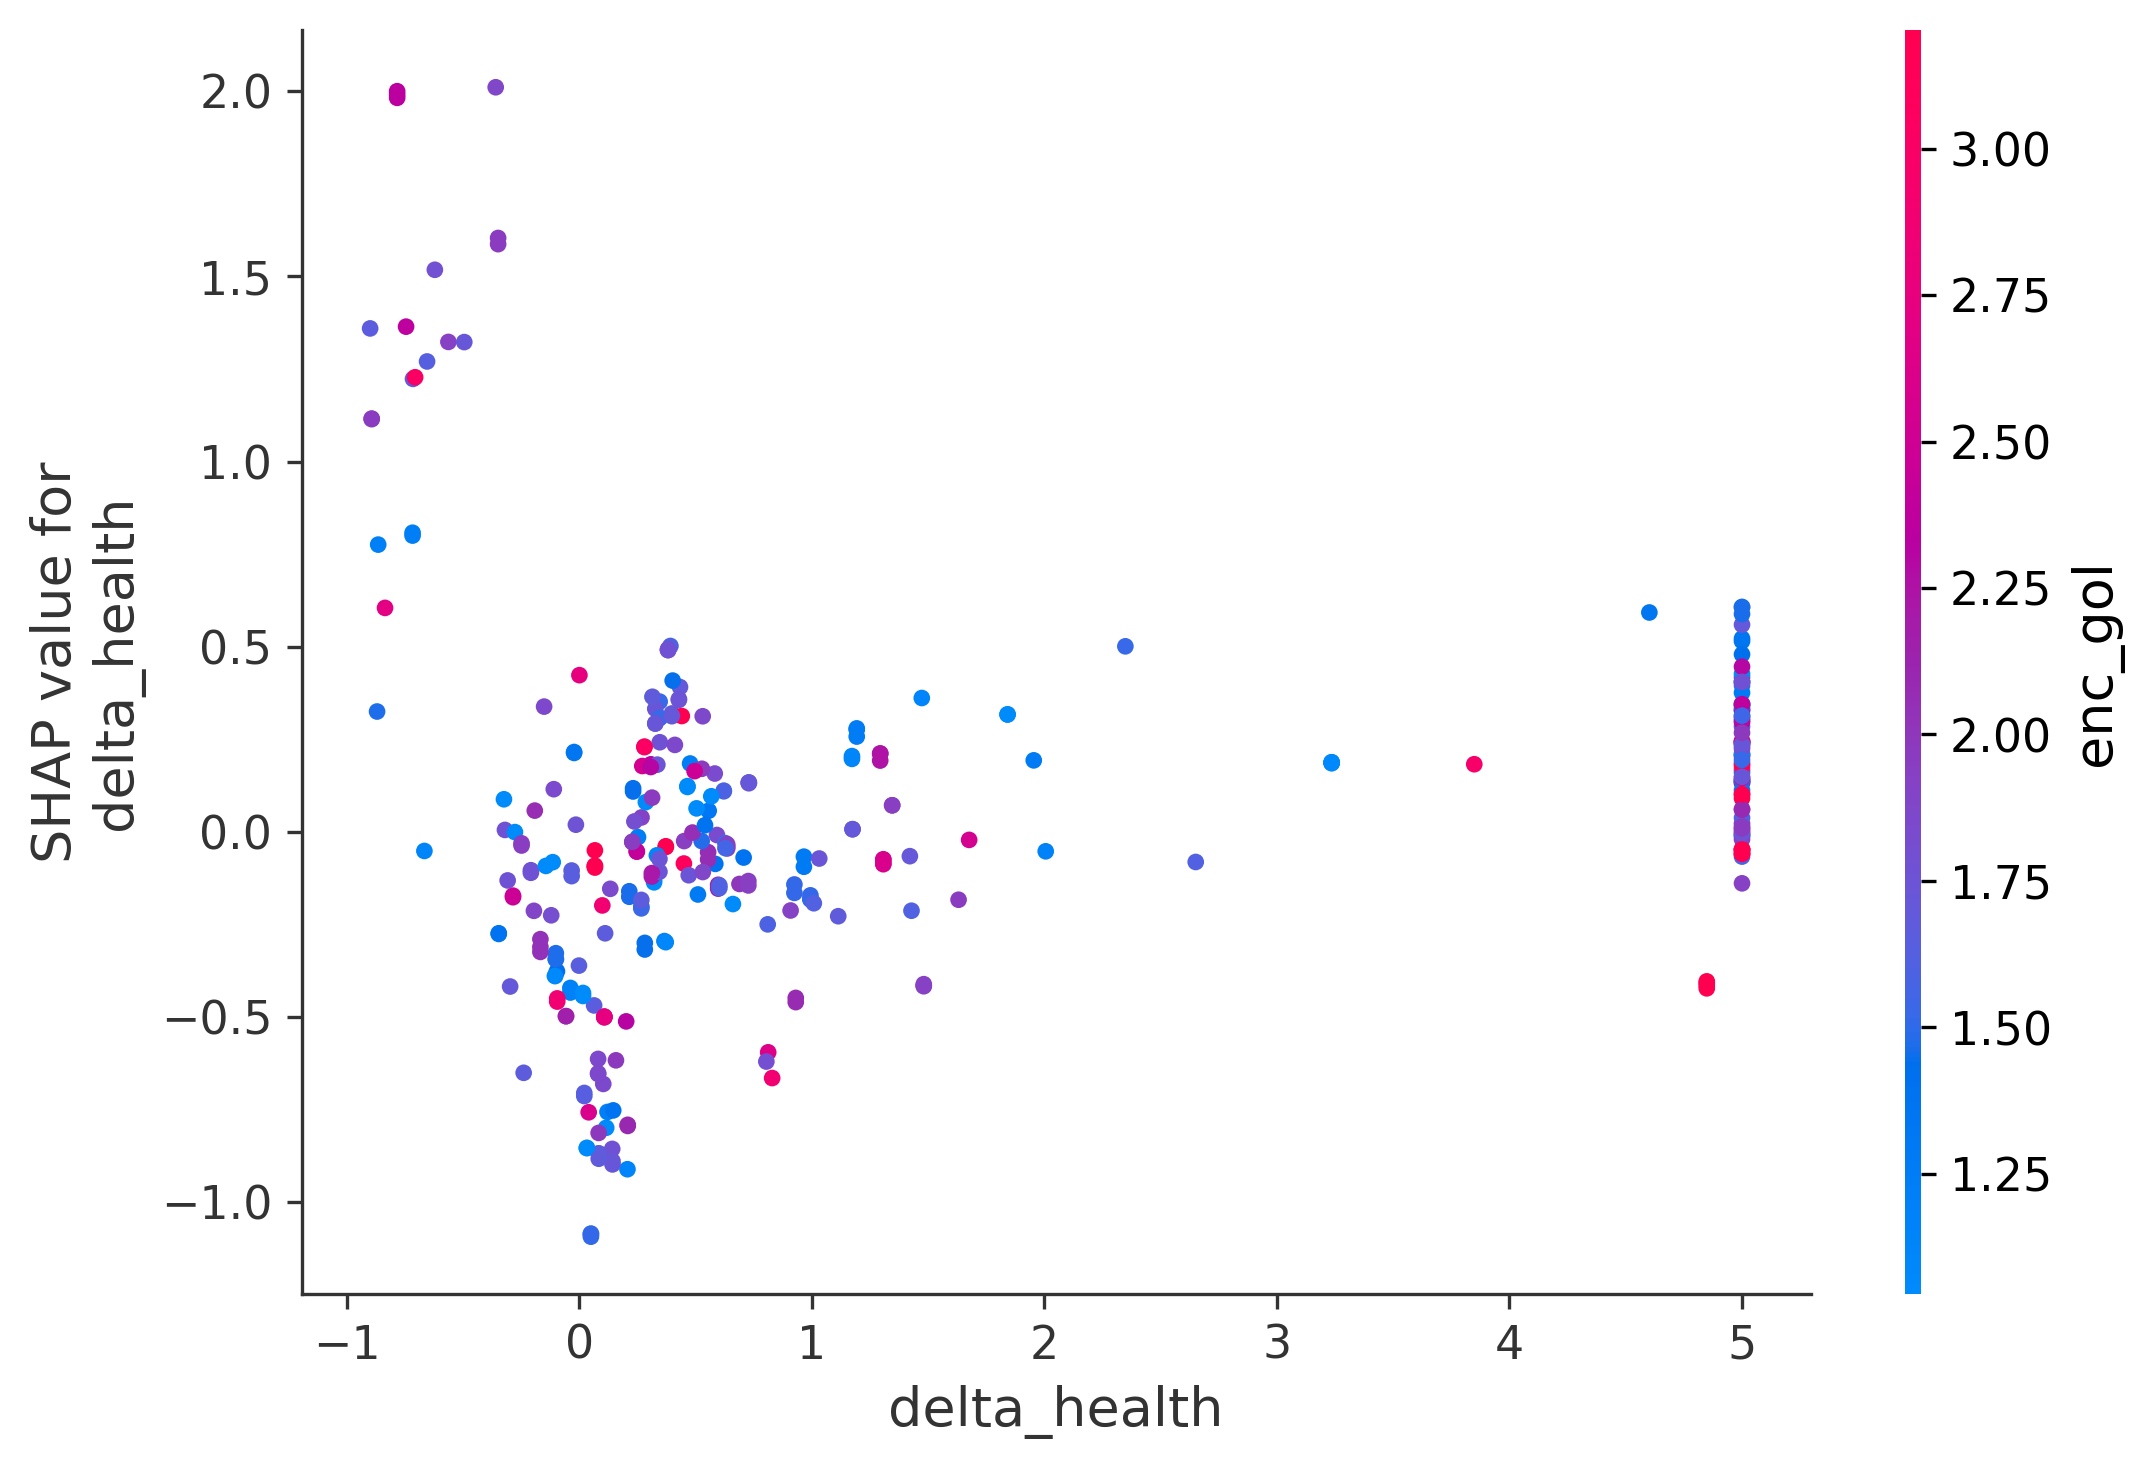
\includegraphics[width=\linewidth]{../data/shap_dependence_health.png}
\caption{SHAP dependence for $\Delta$health.}
\label{fig:shap_health}
\end{subfigure}
\caption{SHAP dependence plots for education and health spending growth.}
\label{fig:shap_dep}
\end{figure}

\subsection{Heterogeneity: Dynasty Interactions}
Table III shows the top features when interaction terms are included. The interaction `dynasty × ∆health` appears at position 9 with gain importance 0.044. Its mean SHAP value (non‑absolute) is 0.020, indicating a small positive effect – dynastic incumbents receive a slightly higher electoral reward for health spending increases. The interaction `dynasty × ∆educ` has a higher mean absolute SHAP (0.252) but lower gain importance, suggesting it is important in some nonlinear way.

\begin{table}[H]
\caption{Top features including interactions (gain importance)}
\centering
\begin{tabular}{lc}
\toprule
Feature & Importance \\
\midrule
region (Cagayan Valley) & 0.064 \\
region (Bicol Region) & 0.064 \\
region (BARMM) & 0.063 \\
region (CALABARZON) & 0.059 \\
region (CARAGA) & 0.051 \\
$\Delta$educ & 0.049 \\
region (SOCCSKSARGEN) & 0.049 \\
dynasty & 0.047 \\
\textbf{dynasty × $\Delta$health} & \textbf{0.044} \\
enc\_gol & 0.042 \\
\bottomrule
\end{tabular}
\end{table}

\subsection{Temporal Robustness}
When trained on pre‑2016 data and tested on 2019–2022, performance drops dramatically: accuracy 44.3\%, AUC 0.412. This indicates that the model does not generalise to future elections.

\subsection{Regression Discontinuity Results}
Table IV presents the RDD estimates for health spending growth. For the 5\% bandwidth, winning a close election increases health spending growth by 1.50 percentage points (95\% CI [0.07, 2.94]). Figure 5 shows the discontinuity plot, and Figure 6 shows sensitivity to bandwidth.

\begin{table}[H]
\caption{RDD estimates (health spending growth)}
\centering
\begin{tabular}{lccc}
\toprule
Bandwidth & ATE & SE & 95\% CI \\
\midrule
3\% & 1.300 & 0.912 & [-0.487, 3.087] \\
5\% & \textbf{1.505} & 0.734 & \textbf{[0.066, 2.943]} \\
7\% & 1.125 & 0.670 & [-0.187, 2.437] \\
\bottomrule
\end{tabular}
\end{table}

\begin{figure}[H]
\centering
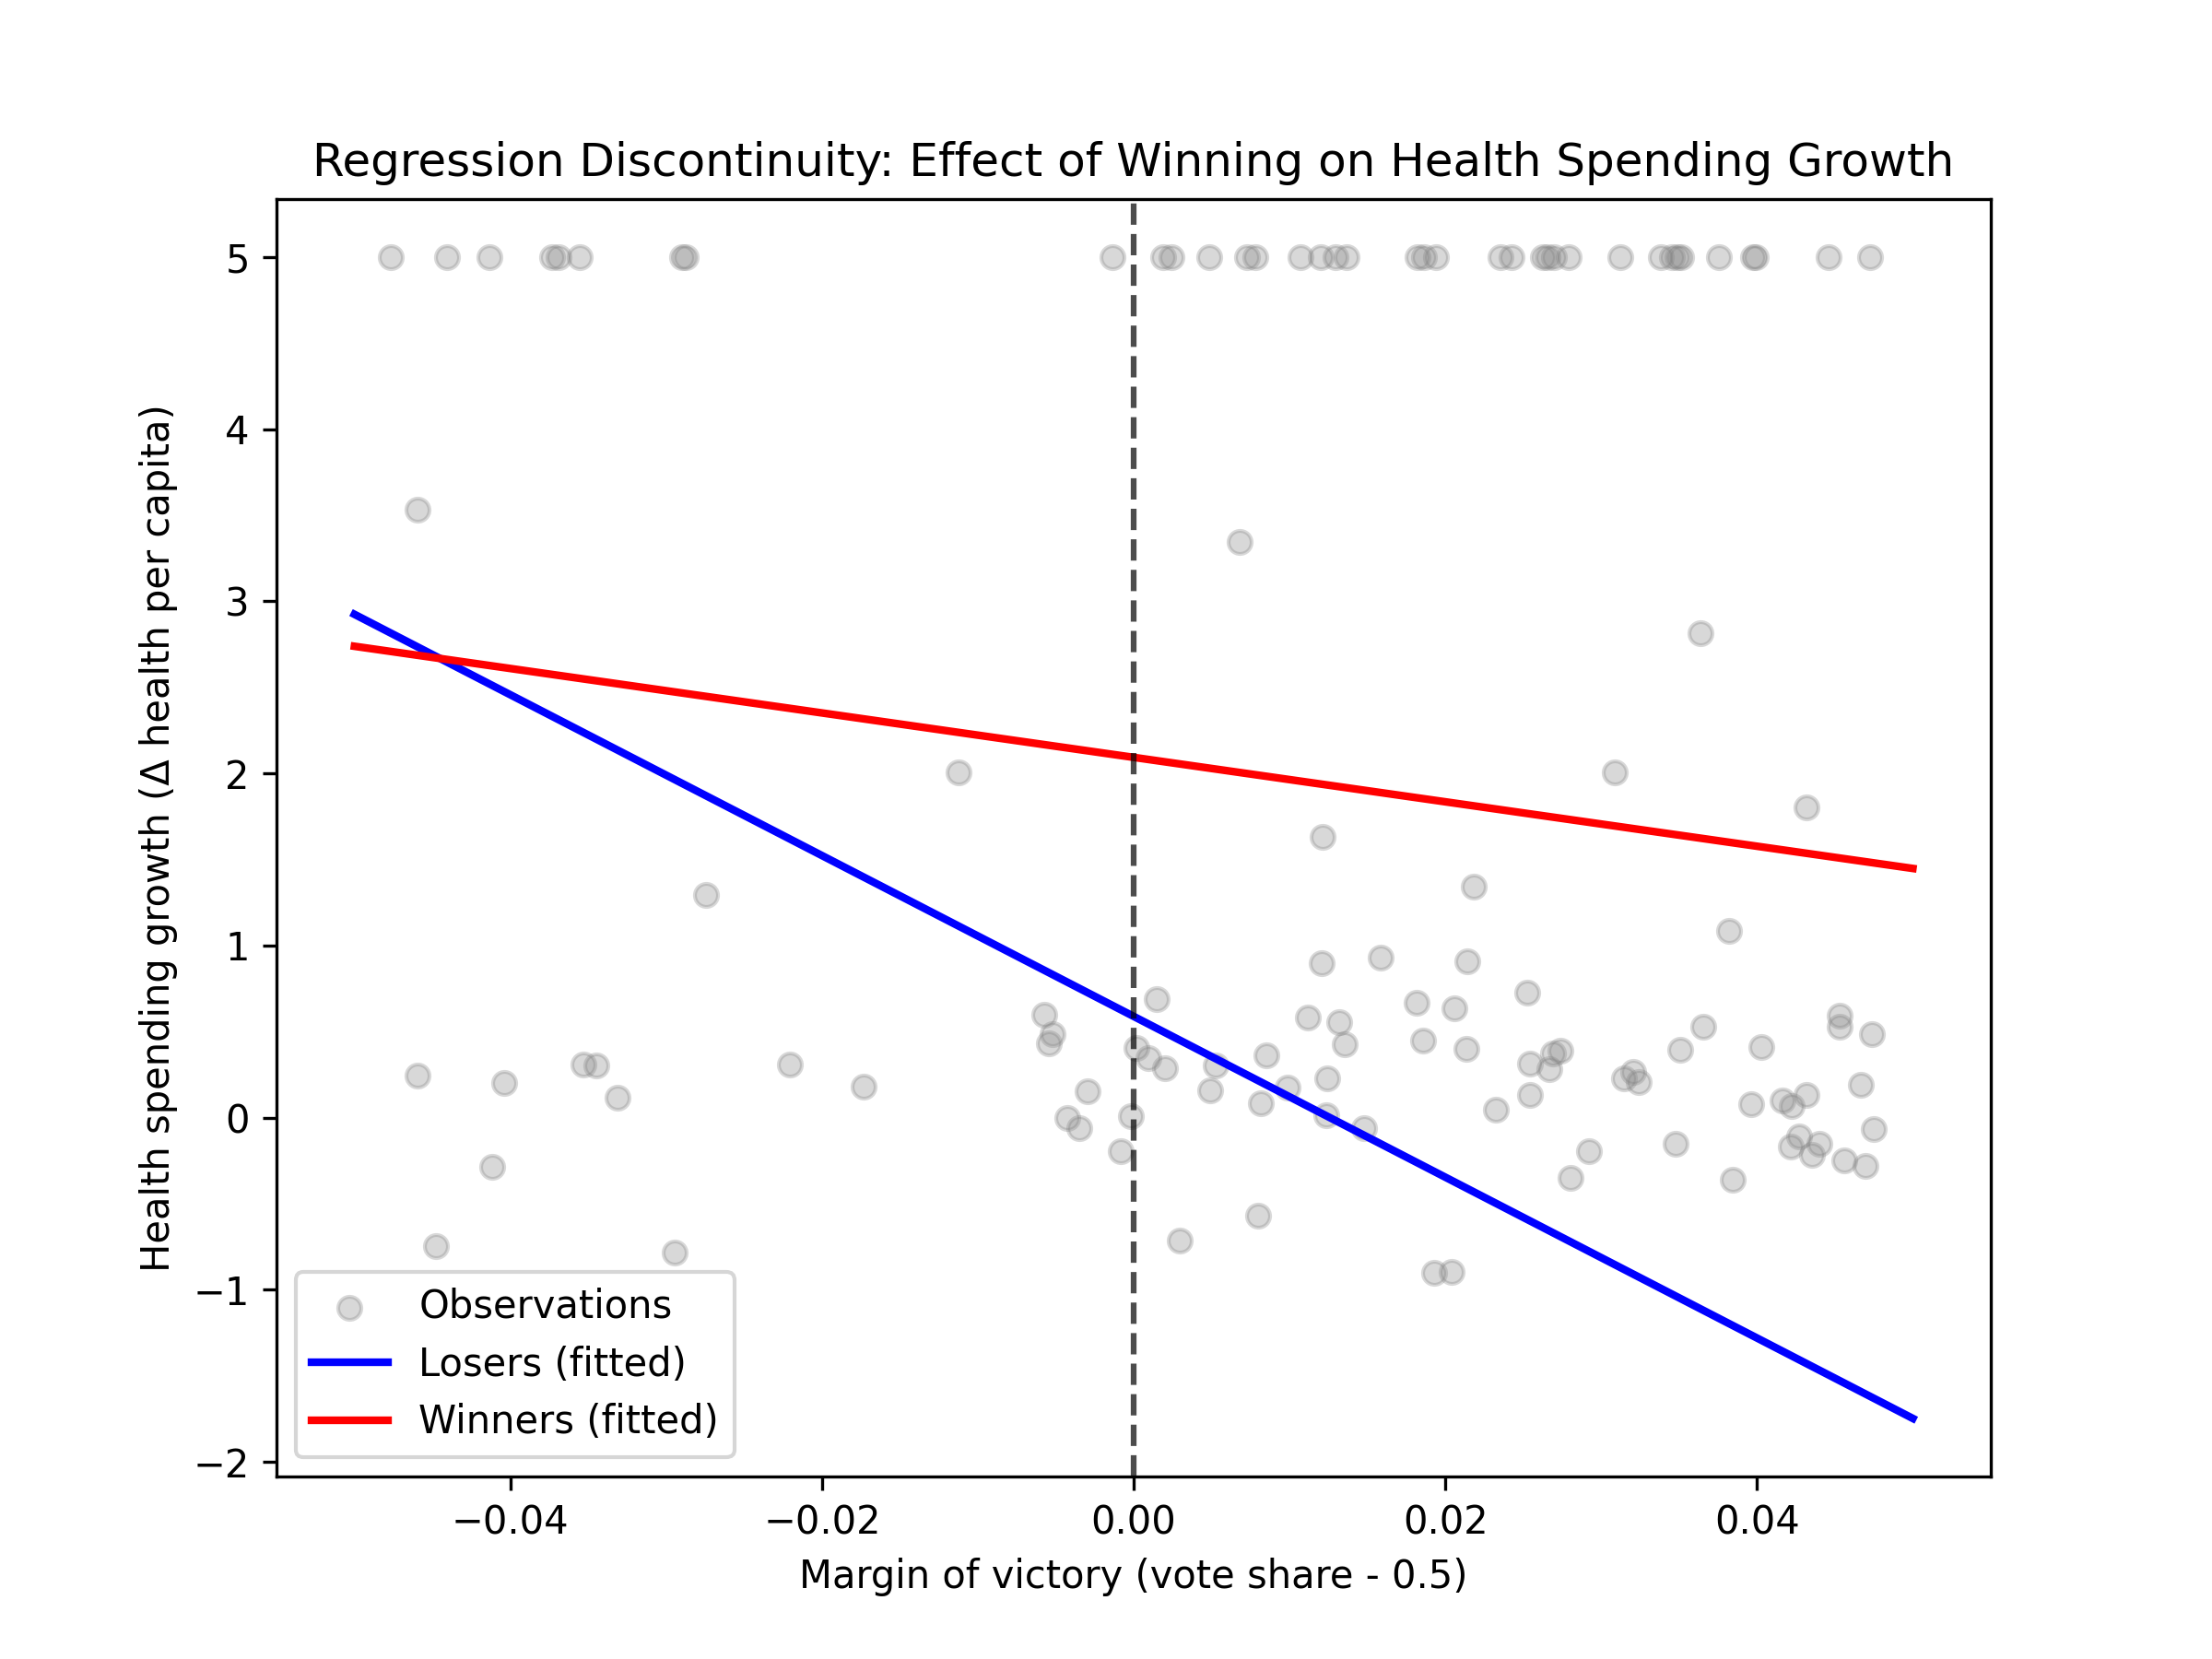
\includegraphics[width=0.9\columnwidth]{../data/rdd_plot.png}
\caption{Regression discontinuity plot (5\% bandwidth).}
\label{fig:rdd}
\end{figure}

\begin{figure}[H]
\centering
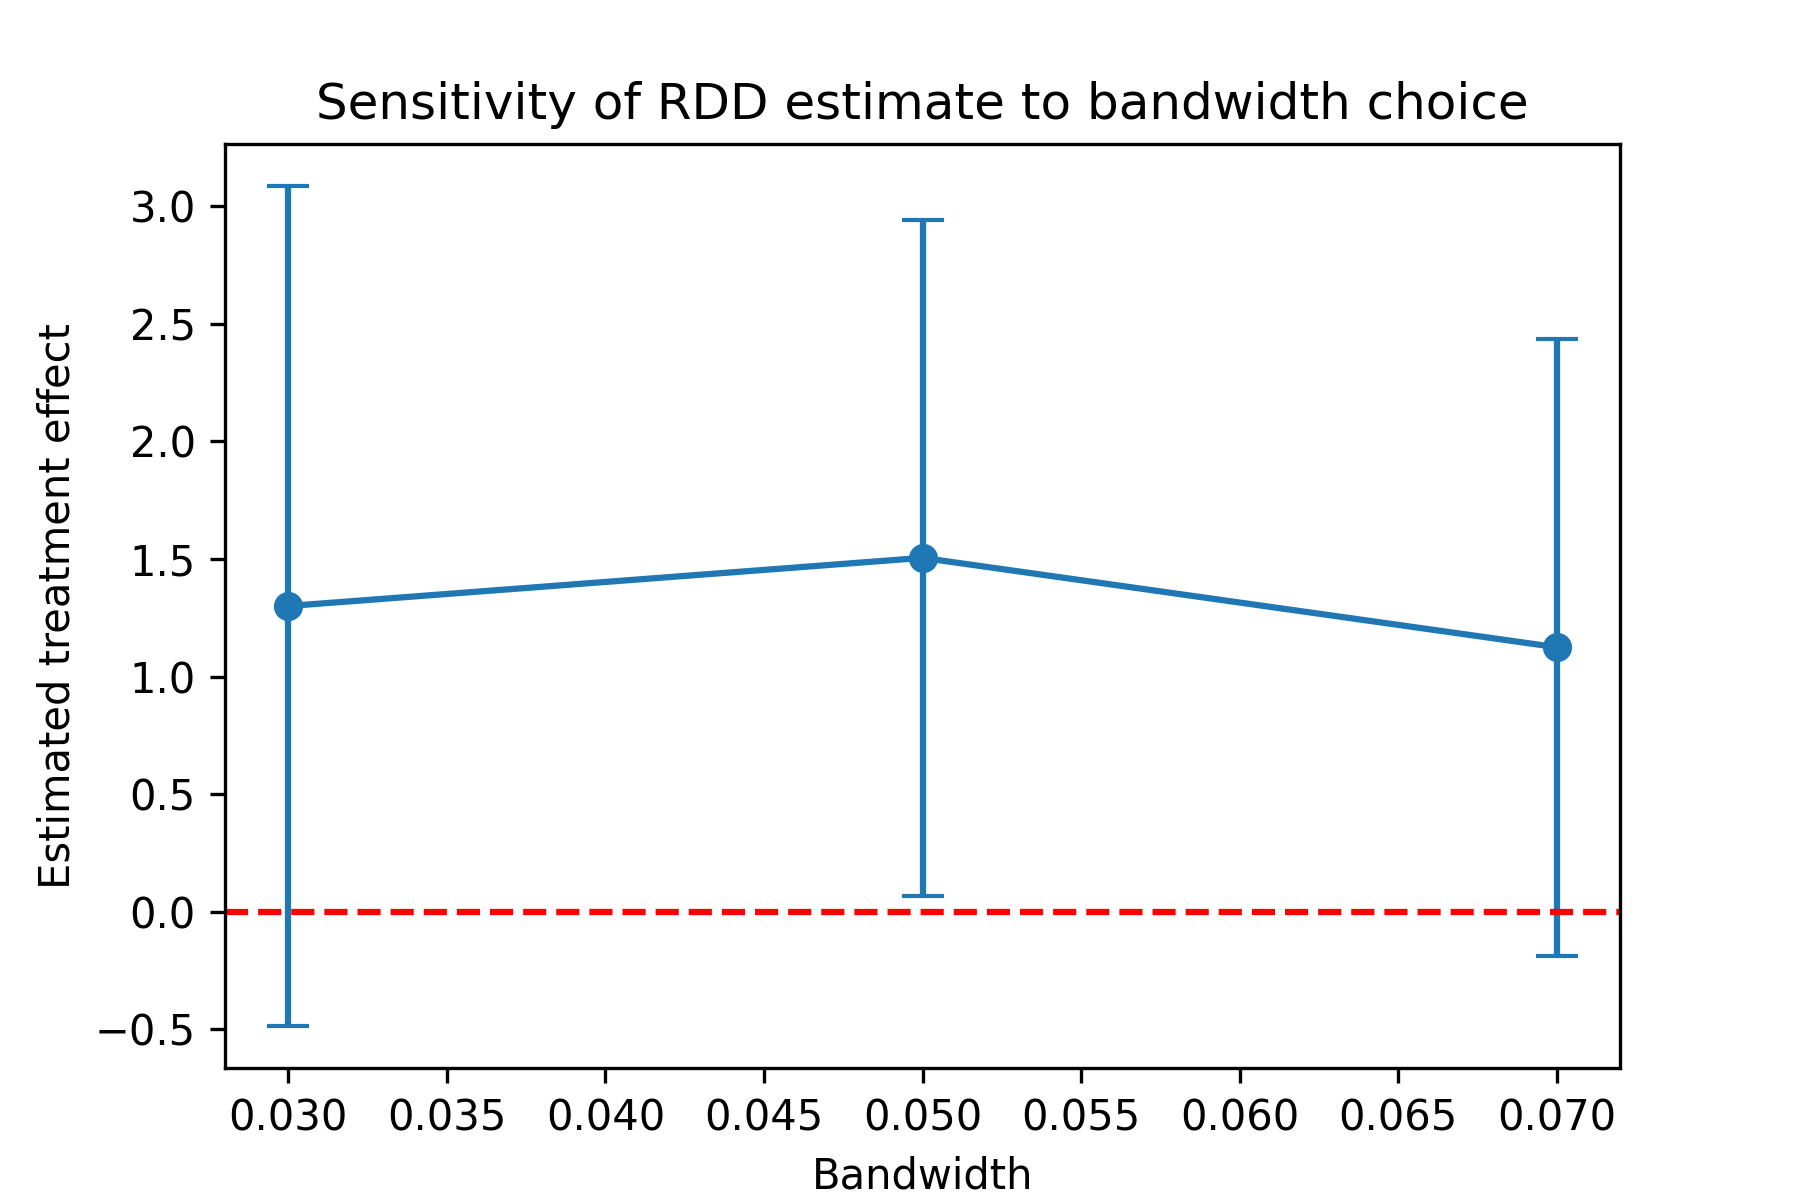
\includegraphics[width=0.9\columnwidth]{../data/rdd_sensitivity.png}
\caption{Sensitivity of RDD estimate to bandwidth choice.}
\label{fig:rdd_sens}
\end{figure}

\subsection{Income Class Subgroup Analysis}
All observations in the final dataset belong to income class 3 (n=1682). The mean SHAP values for this class are: $\Delta$educ = 0.0525, $\Delta$health = 0.0197, dynasty = 0.0062. No comparison between rich and poor provinces is possible. This is a limitation of the sample after merging and cleaning.

\section{Discussion}

The cross‑validated results provide strong evidence that fiscal performance correlates with gubernatorial re‑election in the Philippines. XGBoost consistently outperforms baseline models, and SHAP analysis shows that education and health spending growth positively affect re‑election probability. The dynasty‑by‑health interaction term suggests a small positive effect (mean SHAP 0.020): dynastic incumbents may be rewarded slightly more for health spending than non‑dynastic ones, possibly because they have better political machinery to convert spending into credit. However, the effect size is small, and the interaction with education is less clear.

The temporal failure suggests that the relationship is not stable over time – possibly due to the COVID‑19 pandemic or changing voter priorities. The RDD provides weak causal evidence: winning a close election increases health spending growth, but the effect is only significant at the 5\% bandwidth.

Policy implications:
- \textbf{Invest in education and health:} Voters reward improvements in these sectors.
- \textbf{Local revenue effort:} Increasing local taxes is electorally beneficial (SDG 16).
- \textbf{Dynasties have an advantage:} Anti‑dynasty legislation may reduce incumbency advantage.

\section{Limitations}
\begin{itemize}
\item The predictive model is correlational, not causal.
\item Temporal generalisation fails.
\item The RDD effect is sensitive to bandwidth and only marginally significant.
\item The dataset is limited to governors; mayors may behave differently.
\item Only income class 3 appears in the final sample, preventing heterogeneity analysis by income.
\end{itemize}

\section{Conclusion}
This study demonstrates that fiscal performance correlates with gubernatorial re‑election in the Philippines, with robust cross‑validation metrics (accuracy 92.0\%, AUC 0.977). SHAP analysis shows that education and health spending growth are key drivers. A small positive interaction between dynasty and health spending (mean SHAP 0.020) suggests that dynastic incumbents may be slightly better at converting health spending into votes. However, temporal instability and sample limitations (only one income class) constrain generalisability. The work contributes to SDG 16 (accountable institutions) and SDG 4 (quality education). Future research should incorporate time‑varying effects and larger samples with diverse income classes.

\section*{Acknowledgment}
This paper was originally presented at the 2nd International Conference on the UN SDGs and Social Innovation (ICUNSSI 2026) held on September 23–25, 2026, at the Mindanao State University‑Iligan Institute of Technology, Iligan City, Philippines.

\begin{thebibliography}{99}
\bibitem{b1} J. R. Lott Jr., ``Attendance rates, political shirking, and the effect of post-elective office employment,'' \textit{Economic Inquiry}, vol. 28, no. 1, pp. 133–150, 1990.
\bibitem{b2} L. S. Rothenberg and M. S. Sanders, ``Legislative shirking and electoral accountability,'' \textit{Public Choice}, vol. 103, no. 3/4, pp. 313–335, 2000.
\bibitem{b3} R. U. Mendoza, E. L. Beja Jr., V. S. Venida, and D. B. Yap, ``Political dynasties and poverty: Measurement and evidence,'' \textit{Philippine Review of Economics}, vol. 49, no. 2, pp. 1–25, 2012.
\bibitem{b4} J. J. Capuno, ``Political dynasties and local fiscal performance: Evidence from the Philippines,'' \textit{Asian Journal of Political Science}, vol. 27, no. 2, pp. 123–145, 2019.
\bibitem{b5} R. A. L. Panao, B. F. A. Mendoza, E. F. Habacon, and M. C. C. Reyes, ``Philippine Local Government Interactive Dataset,'' Center for Integrative and Development Studies, University of the Philippines. [Online]. Available: \url{https://elections.cids.up.edu.ph/}
\bibitem{b6} D. S. Lee and T. Lemieux, ``Regression discontinuity designs in economics,'' \textit{Journal of Economic Literature}, vol. 48, no. 2, pp. 281–355, 2010.
\bibitem{b7} V. Chernozhukov et al., ``Double/debiased machine learning for treatment and structural parameters,'' \textit{The Econometrics Journal}, vol. 21, no. 1, pp. C1–C68, 2018.
\bibitem{b8} T. Chen and C. Guestrin, ``XGBoost: A scalable tree boosting system,'' in \textit{Proc. 22nd ACM SIGKDD}, 2016, pp. 785–794.
\bibitem{b9} S. M. Lundberg and S. I. Lee, ``A unified approach to interpreting model predictions,'' in \textit{Advances in Neural Information Processing Systems}, 2017, pp. 4765–4774.
\end{thebibliography}

\end{document}